\section{Atividade 5}

\subsection{Descrição do Modelo e Simulação}
Nesta atividade, simulamos um sistema de controle que envolve um sistema massa-mola-amortecedor com um controlador proporcional. O sistema é descrito pela seguinte equação diferencial:
\[
    m\frac{d^2x(t)}{dt^2} + c\frac{dx(t)}{dt} + kx(t) = f(t),
\]
onde \( m = 10 \), \( c = 7 \), e \( k = 5 \).

\subsection{Construção do Diagrama de Blocos}
O diagrama de blocos para o sistema é apresentado a seguir, ilustrando como os componentes do sistema — controlador, planta e sensor — estão interligados.

\begin{figure}[H]
    \centering
    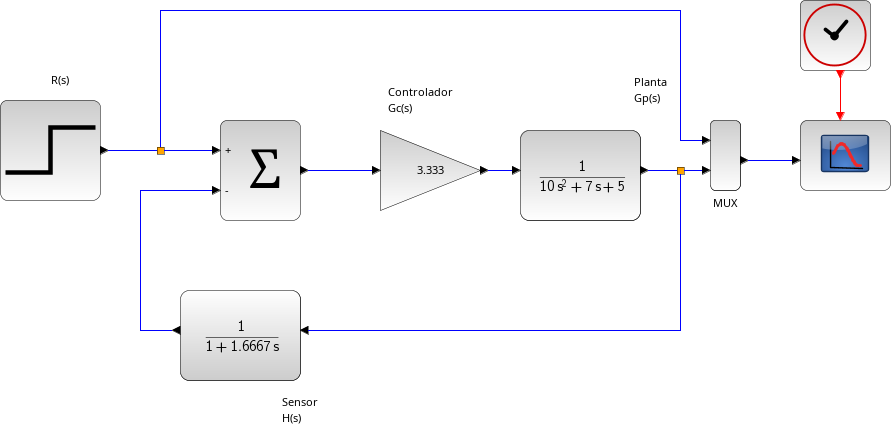
\includegraphics[width=0.7\textwidth]{5-atividade/assets/diagrama-a.png}
    \caption{Diagrama de blocos do sistema de controle para Atividade 5}
    \label{fig:diagrama_blocos_5}
\end{figure}

\subsection{Simulação do Sistema}
Para a simulação, utilizamos um sinal de degrau com amplitude \( A = \frac{m}{4} = 2.5 \). O tempo de simulação foi definido em 50 segundos para permitir a observação completa da resposta do sistema.

\subsubsection{Configuração da Simulação}
O sinal de degrau foi configurado para iniciar em 0 e atingir 2.5 no instante \( t = 1 \) segundo. O tempo de simulação total foi estabelecido para 50 segundos para assegurar que a resposta do sistema fosse completamente observada.

\begin{figure}[H]
    \centering
    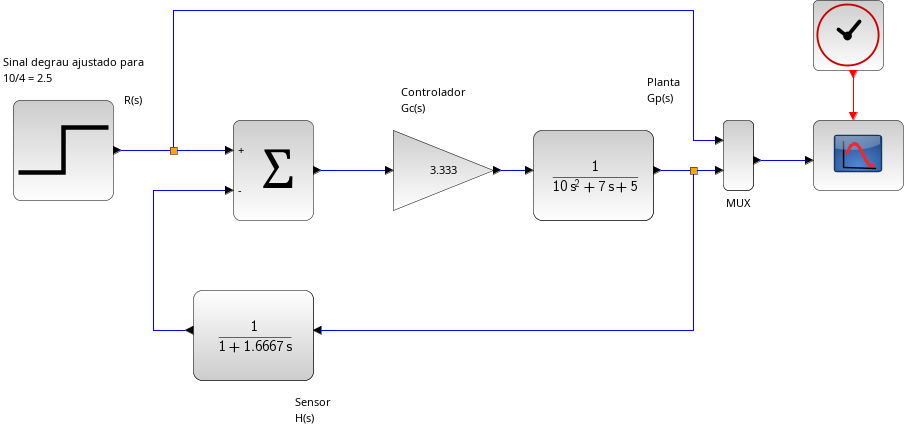
\includegraphics[width=0.8\textwidth]{5-atividade/assets/diagrama-b.png}
    \caption{Diagrama de blocos utilizado para a simulação}
    \label{fig:diagrama_blocos_b}
\end{figure}
\subsubsection{Resultados da Simulação}
A resposta do sistema ao degrau é apresentada na figura abaixo, onde são destacados o tempo de subida, tempo de pico, tempo de acomodação e a zona estacionária, utilizando a ferramenta DataTip para marcar esses pontos significativos.

\begin{figure}[H]
    \centering
    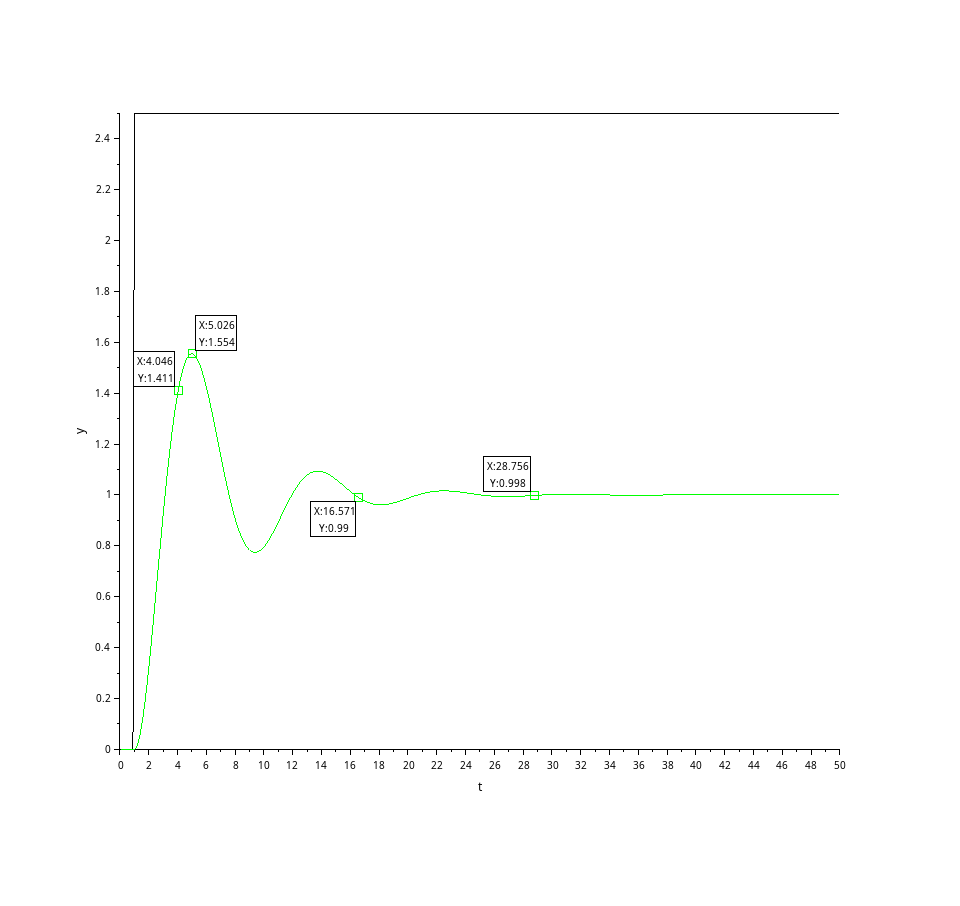
\includegraphics[height=0.7\textwidth]{5-atividade/assets/simulation-b.png}
    \caption{Resposta do sistema ao degrau com configuração de amplitude \( A = 2.5 \)}
    \label{fig:simulation_5b}
\end{figure}

\subsection{Análise Detalhada dos Resultados da Simulação}
A resposta do sistema ao degrau é apresentada na Figura \ref{fig:simulation_5b}, demonstrando as dinâmicas chave do sistema controlado. Analisamos detalhadamente cada parte da resposta:

\begin{itemize}
    \item \textbf{Tempo de Subida:} O tempo de subida refere-se ao intervalo necessário para que a resposta do sistema suba do estado inicial até um determinado percentual do valor final, geralmente 90\%. No gráfico, o sistema leva aproximadamente 4.8 segundos para atingir um valor próximo de 1.55, que é o primeiro pico significativo. Este comportamento inicial mostra como o sistema responde rapidamente ao degrau, com a energia inicialmente absorvida e depois liberada pela combinação de massa, mola e amortecedor.
    \item \textbf{Tempo de Pico:} O pico ocorre no momento em que a saída atinge seu valor máximo em resposta ao degrau. O primeiro pico de 1.55 é atingido em torno de 5 segundos após a aplicação do degrau, ilustrando a máxima extensão da resposta do sistema antes de começar a amortecer devido às forças de fricção e à força restauradora da mola.

    \item \textbf{Tempo de Acomodação:} Após o pico inicial, o sistema começa a se estabilizar, reduzindo as oscilações até alcançar um estado quase constante. Este período é crucial, pois mostra a eficácia do amortecimento em dissipar a energia inicialmente induzida. No gráfico, o sistema mostra sinais de acomodação em torno de 28 segundos, indicando que o amortecimento e a rigidez da mola estão bem dimensionados para controlar as oscilações.

    \item \textbf{Zona Estacionária:} O sistema é considerado em estado estacionário quando as oscilações em torno do valor de equilíbrio se tornam negligíveis. No gráfico, isso é observado após aproximadamente 28 segundos, onde a saída mantém-se constante em cerca de 0.998. Esta fase é fundamental para avaliar se o sistema atingiu o equilíbrio desejado após a perturbação inicial.
\end{itemize}


\textbf{Conclusões da Análise:} A resposta ao degrau revela que o sistema massa-mola-amortecedor, equipado com um controlador proporcional, consegue retornar a um estado de equilíbrio após uma perturbação inicial. A análise destaca a importância de um ajuste apropriado do amortecimento e da rigidez da mola para assegurar que o sistema não apenas retorne ao equilíbrio, mas que o faça de maneira eficiente e sem oscilações excessivas. Este comportamento é indicativo de um sistema bem projetado, capaz de manter a estabilidade mesmo sob condições iniciais desafiadoras.


\subsection{Simulação com Diferentes Configurações de Ganho e Amplitude}
Nesta seção, expandimos a simulação para avaliar o impacto de diferentes configurações de ganho do controlador e amplitude do sinal de entrada. Três casos distintos foram simulados:


\begin{enumerate}
    \item \textbf{Caso Base (Amplitude A=1, Ganho=3.333)}: Mostrado pela linha verde no gráfico.
    \item \textbf{Caso com A=2.5 e Ganho=3.333}: Mostrado pela linha amarela no gráfico.
    \item \textbf{Caso com A=2.5 e Ganho=6.666}: Mostrado pela linha azul no gráfico.
\end{enumerate}

\begin{figure}[H]
    \centering
    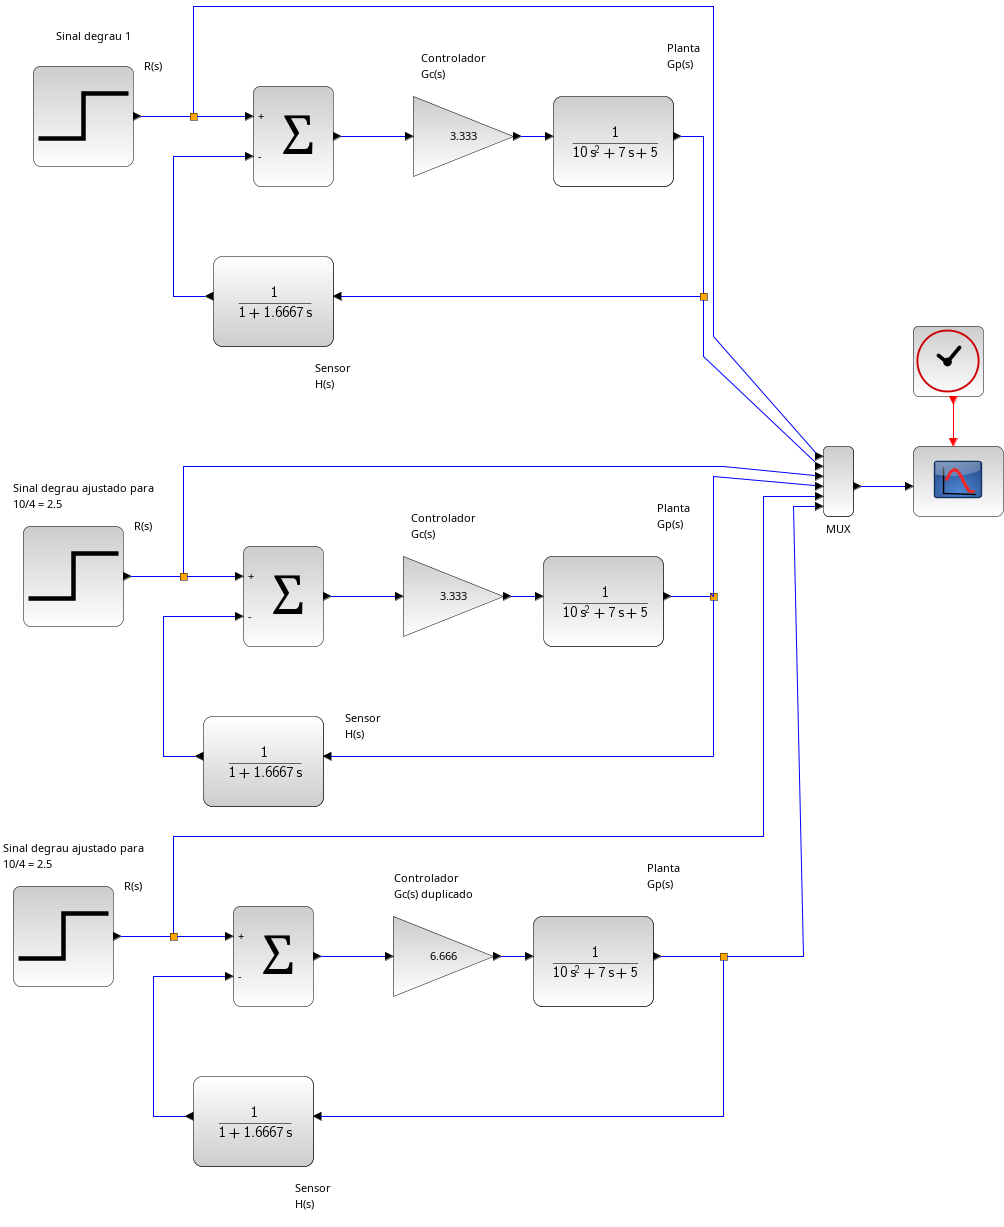
\includegraphics[width=0.8\textwidth]{5-atividade/assets/diagrama-c.png}
    \caption{Diagrama de blocos utilizado para a simulação dos três casos}
    \label{fig:diagrama_blocos_c}
\end{figure}

\subsubsection{Análise dos Resultados}
Os resultados das simulações são visualizados no gráfico seguinte, onde diferentes cores representam os diferentes casos testados.



\begin{figure}[H]
    \centering
    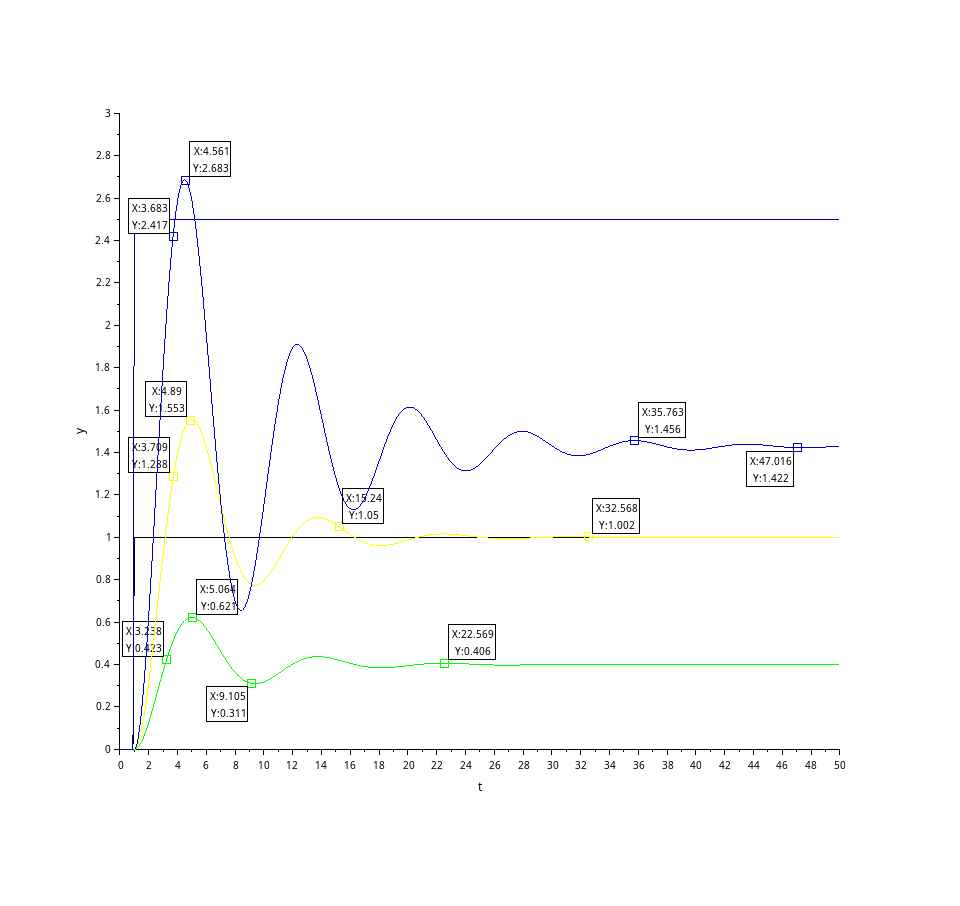
\includegraphics[width=0.8\textwidth]{5-atividade/assets/simulation-c.png}
    \caption{Resposta do sistema para diferentes configurações de ganho e amplitude}
    \label{fig:response_comparison}
\end{figure}

\begin{itemize}
    \item \textbf{Verde (Caso Base)}: A resposta é bastante atenuada, com um pico máximo de aproximadamente 0.311 e acomodação rápida. Este caso mostra a capacidade do sistema de controlar eficazmente pequena perturbações.

    \item \textbf{Amarelo (A=2.5, Ganho=3.333)}: Com o aumento da amplitude, o sistema apresenta um overshoot maior, atingindo aproximadamente 1.554, com oscilações mais pronunciadas antes de estabilizar perto de 1.002. Isso indica que a resposta é mais vigorosa devido à maior entrada, mas ainda gerenciável.

    \item \textbf{Azul (A=2.5, Ganho=6.666)}: O aumento do ganho resulta em um overshoot significativamente maior, cerca de 2.683, com oscilações prolongadas que se estendem ao longo de todo o período de simulação. A resposta é mais agressiva e menos estável, demonstrando que um ganho mais alto pode introduzir instabilidade no sistema.
\end{itemize}

\subsection{Comparação e Comentários sobre as Respostas}
A comparação entre os três casos ilustra claramente a influência da amplitude do sinal de entrada e do ganho do controlador sobre a dinâmica do sistema. As principais observações são:

\begin{itemize}
    \item \textbf{Impacto do Aumento da Amplitude}: O aumento da amplitude do degrau de 1 para 2.5 resulta em um maior overshoot e tempo de acomodação mais longo, o que é esperado em sistemas de controle devido à maior energia introduzida no sistema.

    \item \textbf{Efeitos do Aumento do Ganho do Controlador}: Ao dobrar o ganho do controlador de 3.333 para 6.666, enquanto mantendo a amplitude elevada, observa-se uma resposta muito mais volátil e um pico de overshoot quase dobrado. Isso sugere que embora um ganho mais alto possa ser benéfico para uma resposta mais rápida, também pode comprometer a estabilidade geral do sistema.

    \item \textbf{Conclusões}: Os resultados indicam que um ajuste cuidadoso do ganho é crucial, especialmente em sistemas onde a estabilidade é uma preocupação. Para aplicações que requerem respostas rápidas e podem tolerar algum overshoot, um ganho mais alto pode ser apropriado. No entanto, para a maioria das aplicações industriais e comerciais, um ganho mais moderado e uma abordagem balanceada são recomendados para evitar oscilações excessivas e garantir a estabilidade do sistema.
\end{itemize}

Conclusivamente, esta análise demonstra a importância de um design de controlador bem ponderado, ressaltando a necessidade de equilibrar resposta rápida e estabilidade, dependendo dos requisitos específicos da aplicação.
